	
	The aim of this thesis is to explore the relatively new field of machine
	learning on graphs for the purpose of gaining customer insights. Graph
	machine learning is the current frontier in machine learning and has vast
	applications in many areas as recently shown by the success of AlphaFold
	\citep{senior2020improved}. AlphaFold made a breakthrough for predicting
	protein structures where they made use of the observation that a folded
	protein can be considered as a spatial graph \citep{AlphaFoldTeam2020}. In
	addition, there are a vast range of applications for graphs in the fields of 
	natural science, social science and many more as shown by the excellent 
	overview given by \cite{zhou2020graph}. In principle, graphs are useful 
	whenever one wants to model interactions or relationships. \\

	\noindent From a business \& economics perspective, graphs are particularly
	interesting if one wants to for instance model the interactions between
	institutions. An example for this is a study published by
	\cite{schweitzer2009economic} which created a graph showing the 
	interdependencies of international banks as a network, see figure 
	\ref{fig:bank_network}. This is a useful representation of interdependencies 
	and is an important basis for making systems more robust. \\

	\begin{figure}
		\centering
		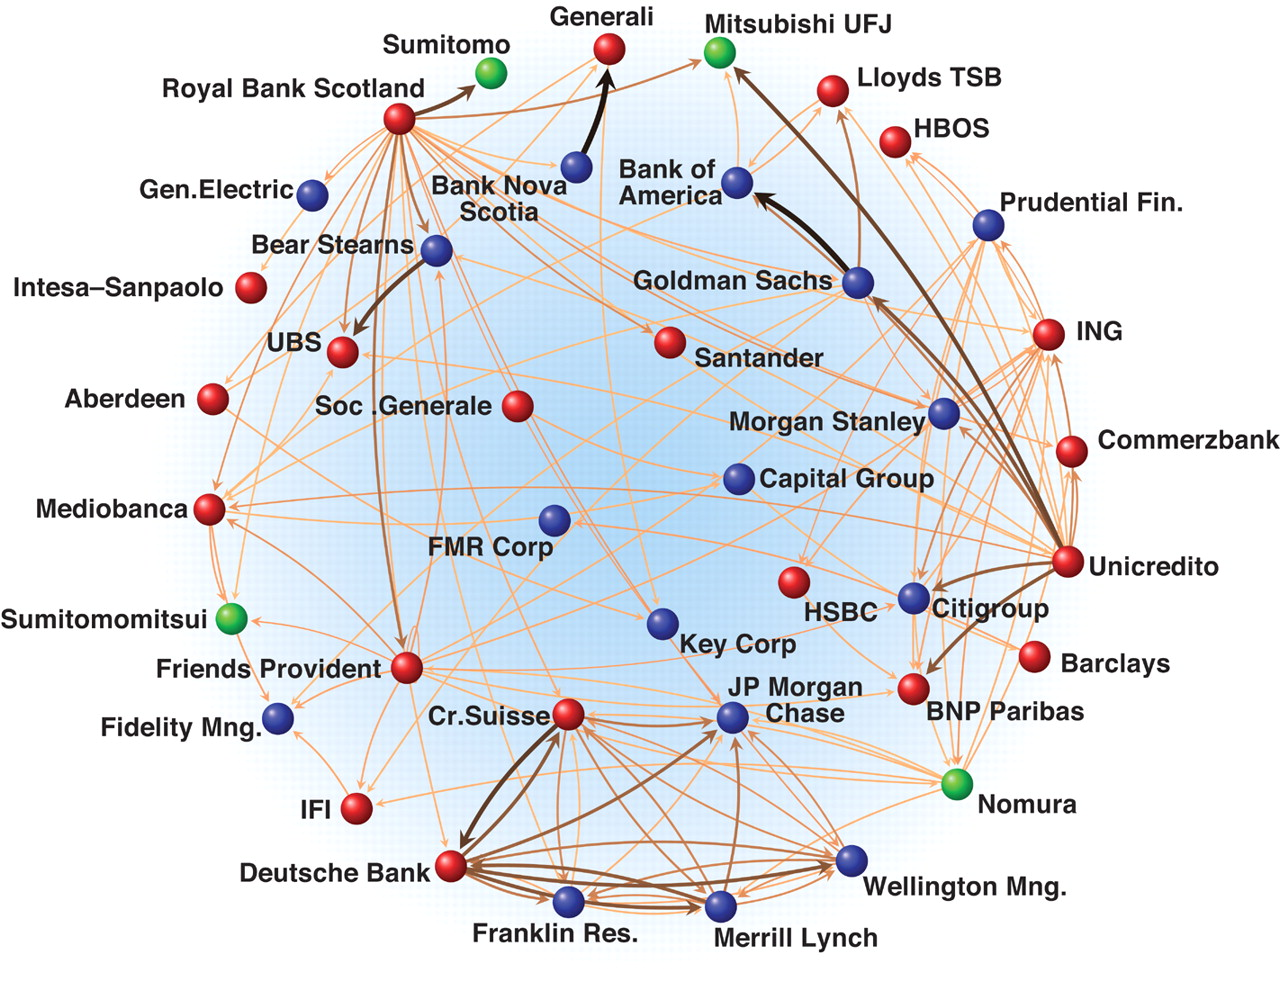
\includegraphics[width=0.5\textwidth]{bank_network.jpg}
		\caption{Bank Network}
		\cite[p. 424]{schweitzer2009economic}
		\label{fig:bank_network}
	\end{figure}

	\noindent Another interesting application of graphs for business \& 
	economics are social interactions. While there are many different types of
	social interactions of interest, social interactions for marketing
	purposes have been among the most popular. Indeed, this is one of the main
	areas where social networks such as Facebook or search providers such as 
	Google make their revenue by selling advertising 
	\citep{Facebook2021,Alphabet2021}.

	\noindent Both Facebook and Google have the advantage, that their businesses
	naturally capture relational or more generally network data which can be
	represented as graphs. Most researchers or companies however do not have 
	access to such data. Companies for instance may have access to large
	amounts of customer data, however they typically would not have access to
	relational information (e.g. which client is connected with which other
	clients). The same is true for researchers, where social scientists
	often collect data via anonymous surveys. This is an issue in terms of data
	access. \\

	\noindent This leads us to the two main aspect of this master thesis which
	consists of:
	
	\begin{enumerate}
		\item Methodology
		\item Application
	\end{enumerate} 

	\noindent Given the difficult access to graph data, this thesis will
	explore whether (semi-) synthetic graphs can be generated using
	cross-sectional data gathered from surveys. The aim is not only to generate
	graphs but to then test whether the resulting graph can be used for
	meaningful machine learning tasks. In order to test this, cross-sectional 
	data of banking clients will be gathered. The aim in terms of application 
	will be to perform an investor classification task. This application area is
	chosen due to the author's experience in this field having worked as a
	client adviser at a bank for over 10 years. One could however choose almost
	any customer classification area, meaning that the application can be chosen
	arbitrarily within reason. \\

	\noindent It would of course be best, if one would have access to real
	graph data. If graph data had been available for a unique application, this
	would have been preferred for this thesis. The absence of such available 
	graph data and the difficulty of generating graph data sparked the interest
	for exploring synthetic graph generation for subsequent machine learning
	tasks. If this application proved to be successful, this could provide an 
	alternative approach for analyzing cross-sectional data. Given the richer
	amount of information.

	\section{Overview Application}

	Retail banking is an area in which client advisers typically serve several 
	hundred if not thousands of clients. In addition, advisers typically work
	in teams which makes personalized advice virtually impossible. For this 
	reason, it is impossible for an adviser to ensure that she provides offers
	to her clients which are in line with their interests. From personal
	experience of the author, having worked as an adviser for over 10 years, 
	this can lead to unsatisfactory outcomes when contacting clients for services or 
	products that they are not interested in. This is largely due to inadequate
	client selection practices. In a bank setting, clients for marketing 
	campaigns, such as promoting investment products, are typically selected based
	on whether they have available liquidity for investment and/or whether a 
	client has already invested in similar products. While this selection makes
	sense to a certain extent, it falls short in that there remain often too 
	many clients in the selection, which are not interested in the offer of a 
	specific marketing campaign or potentially interested clients are falsely 
	excluded in the pre-selection process. \\
	

	\noindent This is an area where classifying clients according to their 
	interests could be of great value and where machine learning methods could 
	be of particular use. It would in addition improve the service quality 
	rendered to clients, prevent unnecessary and perhaps annoying marketing 
	calls and improve the efficiency of a marketing campaigns.
	
	\section{Literature Review}

	There is a lot of published research regarding bank client classification
	using a myriad of methods. Classifications tasks are performed in areas
	such as credit scoring, anti-money laundering (AML) compliance or marketing
	purposes among others
	\citep{sukharev2020ews,weber2018scalable,moro2014data}. \\

	CONTINUE ANOTHER TIME



